\chapter{Background}\label{chap:background}

  \section{Evolution of Image Forgery} \label{sec:s1}
  
Image forgery involves altering the visual contents of an image without leaving traces of the manipulation. This manipulation could be the addition, modification, or removal of any essential features of the image \cite{MeenaTyagi2019}. Image forgery is not a new phenomenon and historically predates the advent of the digital image. In fact, the first forged image in recorded history dates back to the American Civil War in 1860 \cite{Sharma2018AnalysisOK}, 34 years after the invention of photography \cite{Gernsheim_1986}, where a photograph of the politician John Calhoun was manipulated and his body was used in another photograph with the head of the president of the United States, Abraham Lincoln. (Figure \ref{fig:lincon})

\begin{figure}[h!]
  \centering
  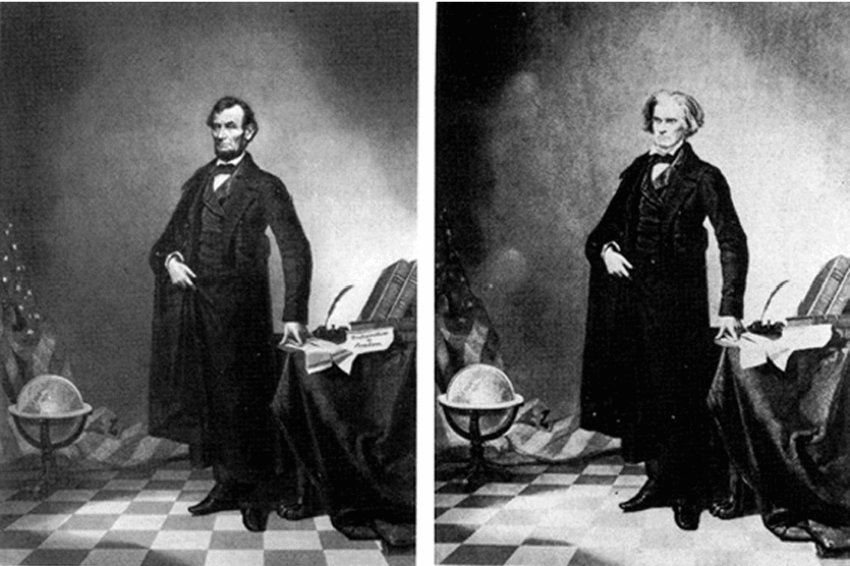
\includegraphics[width=0.5\linewidth]{figures/lincon212.png}
  \caption{The first forged image (left) and the original image (right) \cite{parveen2019}. }
  \label{fig:lincon}
\end{figure}

Numerious previous work in the existing literature \cite{mishra2013digital} \cite{Abdulqader2023} \cite{MeenaTyagi2019} \cite{nampoothiri2016digital} claim that the first `forged' photograph was created in 1840 by French photographer and pioneer Hippolyte Bayard, however this is a misconception. Titled `Self Portrait as a Drowned Man', the image is staged to show him having committed suicide; this was done as an act of frustration towards having lost the title of `Inventor of Photography' to Louis Daguerre, who patented the process before him (Figure \ref{fig:drowned} ). The error in this claim lies in the fact that this is, in fact, the first `staged' image and not the first forged image, since the deception occurred before the creation of the image where in contrast forgery typically involves manipulating an existing image. 

\begin{figure}[h!]
  \centering
  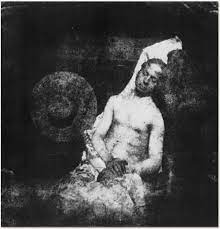
\includegraphics[width=0.4\linewidth]{figures/drownedman.jpeg}
  \caption{Self Portrait as a Drowned Man, the first staged image. \cite{bayard}}
  \label{fig:drowned}
\end{figure}


When it comes to pinpointing the first instance of digital image forgery, the task becomes quite challenging due to the lack of a widely accepted definition for what constitutes a digital forgery during the days of early digital imaging. Early experiments and forgeries in the field of digital art and computer graphics took place in educational and research environments, therefore an accurate answer is difficult to find. Despite there not being an official `first digital forgery' there are early notable instances, one being the `O.J. Simpson Time Magazine cover' from 1994  \cite{Carmody_1994}, where Simpson's skin tone was allegedly darkened on the magazine's cover to make him appear more menacing. This incident raised ethical concerns about the manipulation of images in journalism.

\begin{figure}[h!]
  \centering
  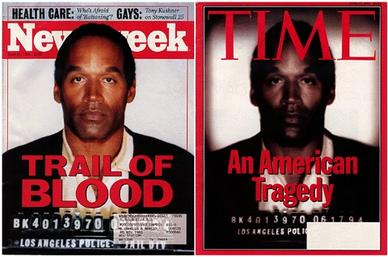
\includegraphics[width=0.5\linewidth]{figures/oj_simpson.jpg}
  \caption{O.J. Simpson on the covers of Newsweek and Time Magazine. The picture on the right was altered to make Simpson appear darker. \cite{OJ2011}}
  \label{fig:drowned}
\end{figure}

In the late 20th century, photography greatly evolved into the digital realm, and the advent of graphic imaging software such as Adobe Photoshop or GIMP made digital retouching and editing possible \cite{Peres_2007}. The skill-intensive and time-consuming nature of using these programs, which were the only options available at the time, made the probability of a proliferation in image forgeries unlikely. Eventually, technical advancements of the 21st century and advent of deep learning created a new wave of image editing software that is powered by advanced algorithms which allow complex transformations to be mostly automated \cite{corcoran2014}. Nowadays, a number of popular social media apps, like Instagram and TikTok, offer beauty filters which may also be applied in real-time to live video. These filters smooth skin tones and generate more visually pleasing face proportions (for example, by enlarging a subject's eyes). Applications for mobile image editing, such as Facetune, also offer these features. Some, like FaceApp, automate intricate, content-aware alterations, such altering the subject's age or gender or their facial expression, using deep learning algorithms \cite{Vincent_2017}. The ease of use and availability of these technologies, often for free, led to a distrust in the authenticity of visual information, especially on social media.\cite{perez2021fake} The proliferation of image forgeries was no longer a matter of probability, but became a reality. 

The year 2017 saw the emergence and spread of `Deepfakes', a form of synthetic media in which artificial intelligence (AI) and deep learning techniques are used to create or manipulate audio and visual content to make it appear as though someone is saying or doing something they did not \cite{kietzmann2020deepfakes}. The term `deepfake' originated from a Reddit user called `deepfake' who was known for sharing the deepfakes he created; many videos involved celebrities' faces swapped onto the bodies of actresses in pornographic videos \cite{Cola_2018}. The term is a portmanteau of `deep learning' and `fake'. One major problem is how deepfakes contribute to fake news. The potential to produce extremely convincing and misleading videos increases the likelihood of misinformation and disinformation spreading \cite{Fallis_2020}. Deepfakes create the impression that prominent individuals are saying or doing things they never did, which can be exploited to sway public opinion, harm people's reputations, or affect political outcomes. By 2020, audio deepfakes had emerged \cite{muller2022human}, and AI software capable of both creating and detecting deepfakes, including cloning human voices after just five seconds of listening time, became available. Impressions, a mobile deepfake app, launched in March 2020, pioneering the creation of celebrity deepfake videos directly from mobile phones \cite{Mathews2020}.

As briefly explored above, image manipulation has been used to deceive or persuade viewers or, more lightheartedly, improve storytelling and self-expression. It then becomes clear that image manipulation is not inherently malicious and it is, in fact, the intent, the nature of the manipulation, and its consequences that determine whether the manipulation can be considered a malicious forgery. This, in turn, allows us to create a consistent definition of what forgeries are and how to classify them, aiding in the task of detecting them and mitigating their spread.

According to a survey done by Meena and Tyagi \cite{MeenaTyagi2019}, the act of image forgery itself can be classified into two types: content-preserving or content-altering forgery. Content-preserving forgery includes operations such as geometric transformation, changing the format, enhancement, etc. Content-altering forgery involves altering the content of digital images to misinterpret and mislead the information conveyed by the image, ie. its semantic meaning. As such, one form of tampering can be seen as more malicious than the other. Retouching and resampling are examples of legitimate content-preserving tampering that tries to improve visual appeal or resize photos for specific purposes like magazine covers or social media. Most of the time, these modifications are generally accepted and harmless. On the other hand, content-altering tampering is seen as malicious and illegal tampering as it attacks an image’s semantic integrity. 

Traditionally, the two primary types of illegal tampering, in which parts are joined or altered to purposefully trick and mislead viewers, are copy-move forgery and image splicing forgery \cite{Lian2010}. Copy-move forgery involves duplicating and placing one part of an image onto another to create a false appearance of objects being in multiple locations. Image splicing, as shown in Figure \ref{fig:splice}, is a manipulation technique where different parts of multiple images are combined to create a deceptive composite image. Deepfakes can be considered the new, third type of illegal tampering as they do not fall under the categories of either copy-move or image splicing. 

  \section{Digital Image Forensics} \label{sec:s2}

Image forgery detection refers to the process of identifying manipulations or alterations in digital images that are intended to deceive or mislead. The goal is to distinguish between authentic images and those that have been tampered with, ensuring the integrity and reliability of visual content \cite{MeenaTyagi2021}. Image forgery detection techniques are broadly classified into two categories: active and passive. Active forgery detection requires prior embedded information about the query image, which can be added during image acquisition or later using hardware or software. The embedded data is then extracted from the query image to assess the likelihood of forgery. This data is mostly embedded in the form of a watermark or a digital signature.\cite{zanardelli2023image} However, active forgery detection has limitations when applied to photographs from the Internet or social media, as these images lack embedded information. In response, passive forgery detection methods have been developed, operating without prior knowledge of the query image.\cite{MeenaTyagi2021}

Digital forgeries leave almost no visual clues with regard to tampering, but the image structure is disturbed, which introduces new artifacts resulting in various forms of inconsistencies \cite{Lian2010}. Passive methods, also known as Digital Image Forensics (DIF), rely on the application of forensic techniques to analyze these inconsistencies in the digital image to detect the forgery\cite{FERREIRA2020106685}. Image forgery detection is a two-class (binary) classification problem. The objective of a DIF model is to classify a given image as either authentic or forged. As shown in Figure \ref{fig:framework}, the general framework of the existing DIF approaches includes extracting representative and relevant features from an image first, then a suitable classifier is trained and modeled by using the features, and finally classification is performed by using the trained model. 

\begin{figure}[h!]
  \centering
  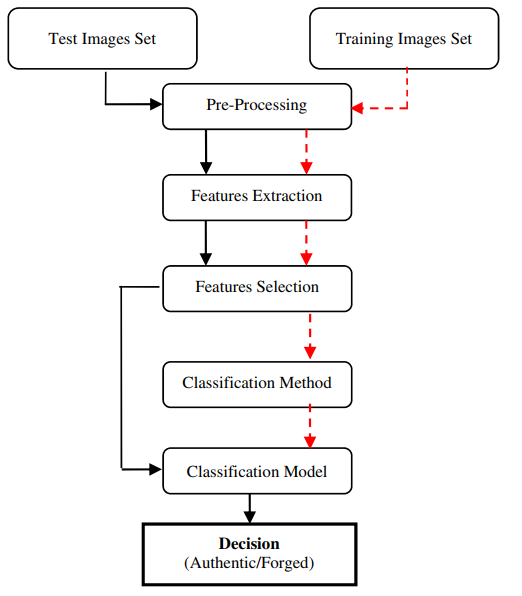
\includegraphics[width=0.5\linewidth]{figures/DetectionWorkflow.png} % Replace "example-image" with the filename of your image
  \caption{General Framework for forgery detection.}
  \label{fig:framework}
\end{figure}

Figure \ref{fig:imgauth} shows how the passive DIF is categorized into forgery-dependent approaches and forgery-independent approaches.Forgery-independent techniques concentrate on finding irregularities or inconsistencies within the image itself, while forgery-dependent techniques rely on particular forgery features and assumptions about the alteration process \cite{Basavaraj2022}. Forgery-independent techniques by definition have a wider use but may have some limits in terms of false positives or the identification of complex forgeries, meanwhile forgery-dependent strategies can be effective when the forgery process is known.

\begin{figure}[h!]
  \centering
  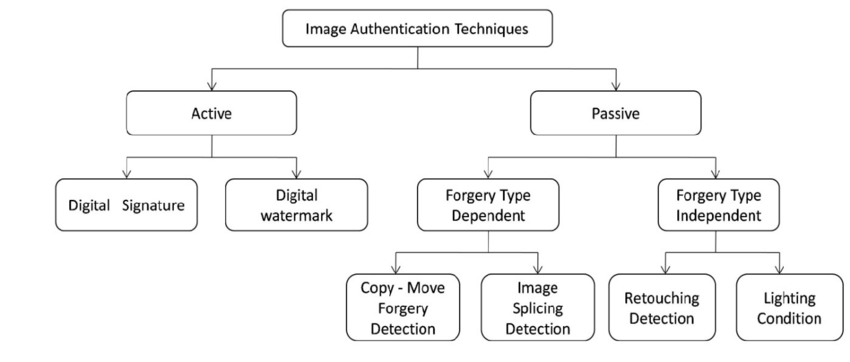
\includegraphics[width=0.8\linewidth]{figures/ImageAuthenticationGraph.png} % Replace "example-image" with the filename of your image
  \caption{Classification of  image authentication techniques. \cite{alahmadi2017passive}}
  \label{fig:imgauth}
\end{figure}

As mentioned in the previous section, the three main types of illegal tampering are copy-move, image splicing and deepfakes. Consequently, the majority of effort and research done in the field of DIF is focused on these forgery techniques \cite{zanardelli2023image}. However, as observed in many review and survey papers \cite{MeenaTyagi2021}, there are relatively few approaches dedicated to detecting image splicing compared to copy-move forgery detection (CMFD) and deepfakes; this represents a gap in the research, and therefore, image splicing detection techniques are the focus of this thesis and will be highlighted in the related works section. 

\begin{figure}[h!]
  \centering
  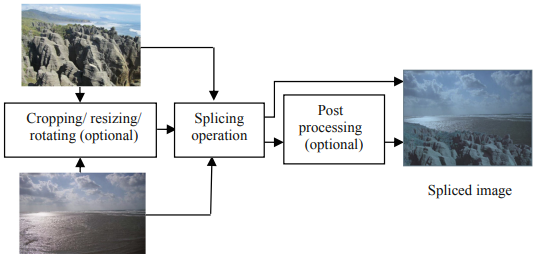
\includegraphics[width=0.7\linewidth]{figures/StepsToSplice.png}
  \caption{Steps to creating a spliced image. \cite{MeenaTyagi2019}}
  \label{fig:splice}
\end{figure}

  \section{JPEG Compression \& Image Forensics } \label{sec:s3}


JPEG (Joint Photographic Experts Group) stands as a widely embraced image compression standard, celebrated for its efficiency in storing and transmitting digital images. Its popularity stems from the ability to achieve notable compression ratios while preserving acceptable image quality. \cite{wallace1992jpeg} This algorithm, widely utilized in various applications such as digital photography, web content, and social media, achieves compression by removing redundant information and approximating image data. The adaptability of JPEG, allowing for an adjustable tradeoff between storage size and image quality, further cements its dominance in the digital imaging landscape, supported by widespread compatibility \cite{palmer2013rhetoric}.

Being the default and most widely supported format for image storage and sharing on the internet, JPEG plays a pivotal role in the digital realm. The majority of digital cameras, smartphones, and image-sharing platforms employ JPEG compression, making it integral to the fabric of online visual content.

However, this widespread usage has inadvertently led to concerns related to image forgery, especially in the context of image splicing. JPEG compression, while achieving efficient file sizes, introduces artifacts during the compression process. Lossy compression sacrifices specific image details and may result in the smoothing of high-frequency components. The Discrete Cosine Transform (DCT) and blocking artifacts at block boundaries, coupled with quantization errors, contribute to distinctive patterns within the image. Forgers adeptly utilize these compression artifacts to conceal seams between spliced regions during image manipulation \cite{Ma_Jiang_Fan_Jiang_Yan_2020}. This strategic use makes it challenging for traditional forgery detection methods to discern the manipulation. Consequently, advanced splicing techniques are continually evolving to effectively conceal these artifacts, fueling ongoing research into sophisticated forgery detection methods.

The ubiquity of JPEG images on social media platforms renders them susceptible to the dissemination of manipulated or forged images, accentuating the potential for the spread of disinformation. Disinformation campaigns leverage manipulated images to shape public perception, spread false narratives, and create misleading visual evidence. JPEG splicing, enabling the creation of realistic yet fabricated images, stands as a potent tool for deception and misinformation in this digital age \cite{huh2018fighting}. As a result, the detection of forgeries in JPEG images especially is a thriving branch of digital image forensics and therefore, the contributions of this work are mainly targeted at addressing the splicing of JPEG images.


  \section{Deep Learning in Digital Image Forensics} \label{sec:s4}

Machine learning, a subset of AI, empowers systems to learn and improve from experience without explicit programming. Deep learning is a branch of machine learning that involves the use of neural networks with multiple layers (known as deep neural networks) to analyze and learn patterns from vast amounts of data \cite{campesato2020artificial}. The journey of deep learning commenced with the development of artificial neural networks, inspired by the structure and functioning of the human brain. These networks are capable of automatically extracting hierarchical features and representations, making them highly effective in tasks such as image recognition, classification, and pattern detection \cite{nielsen2015neural}.

The use of deep learning in image forensics represents a more recent development, leveraging the capabilities of these advanced algorithms to detect and analyze digital image manipulations. The integration of deep learning techniques in image forensics gained traction as computational power increased, allowing for the training of complex neural networks on large datasets \cite{rota2016bad}.

  \subsection{Convolutional Neural Networks} \label{ssec:s1}

The concept of convolutional neural networks (CNNs) is inspired by the human visual system. It was introduced in a landmark paper titled `Gradient-Based Learning Applied to Document Recognition' by Yann LeCun et. al in 1998 \cite{lecun1998gradient}. The paper proposed the LeNet-5 architecture, specifically designed to recognize handwritten digits in checks and postal codes, demonstrating the effectiveness of CNNs in learning hierarchical features from input data. This work marked a groundbreaking milestone in the history of deep learning and became foundational for subsequent applications in computer vision, including image forensics.

CNNs revolutionized computer vision by addressing the spatial hierarchies within images. The architecture of CNNs mimics the human visual system, employing convolutional layers to recognize local patterns, pooling layers to downsample, and fully connected layers for classification \cite{lindsay2021convolutional}. The success of CNNs in tasks like image recognition, object detection, and segmentation solidified their status as the go-to architecture in the realm of computer vision \cite{bhatt2021cnn}. These networks excel at feature extraction, capturing hierarchical representations of input data. The convolutional layers apply filters to detect low-level features like edges and textures, gradually combining them to identify more complex patterns \cite{bhatt2021cnn}. CNNs' efficacy in image classification is exemplified by their deployment in renowned architectures like AlexNet \cite{alom2018history}, VGGNet \cite{majib2021vgg}, and ResNet \cite{targ2016resnet}, setting benchmarks in various computer vision competitions.

While CNNs thrived, their reliance on fixed-size grids and limited global context became apparent challenges \cite{Ahmed_Alam2023}. The breakthrough in natural language processing with transformers, as showcased by models like BERT and GPT, inspired researchers to explore their potential in computer vision \cite{WANG2023100047}.

  \subsection{Vision Transformers} \label{ssec:s2}

Vision Transformers (ViTs) emerged as a groundbreaking architecture for computer vision, challenging the conventional dominance of Convolutional Neural Networks (CNNs). The ViT model, introduced in the paper `An Image is Worth 16x16 Words: Transformers for Image Recognition' by Alexey Dosovitskiy et al., marked a significant departure from grid-based processing, treating images as sequences of fixed-size patches \cite{dosovitskiy2021image}.

At the heart of ViTs is the transformer architecture, initially designed for natural language processing tasks. ViTs, however, adapt this architecture to handle visual data by dividing an image into non-overlapping patches, which are then linearly embedded into high-dimensional vectors. These patch embeddings serve as the input tokens for the transformer model \cite{ruan2022vision}.

The transformer consists of two main components: the encoder and the decoder. In ViTs, only the encoder is used \cite{ruan2022vision}. The encoder comprises multiple layers, each containing self-attention mechanisms and feedforward neural networks. The self-attention mechanism enables the model to capture relationships between different patches, allowing for the extraction of global contextual information. The model learns to attend to relevant patches while suppressing irrelevant ones, effectively achieving a holistic understanding of the image \cite{islam2023recent}.

\begin{figure}[h!]
  \centering
  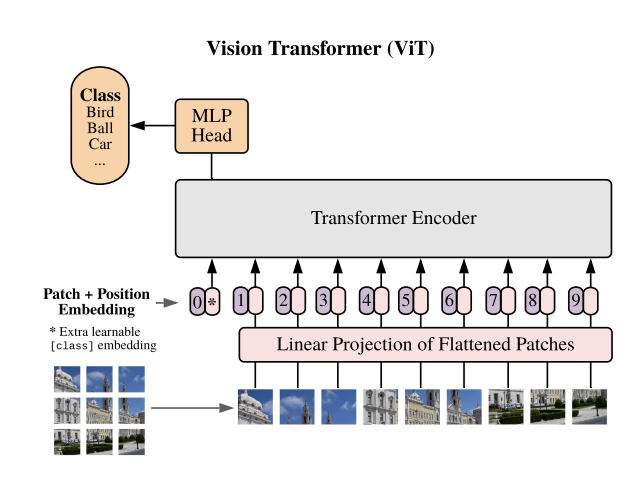
\includegraphics[width=0.8\linewidth]{figures/Vit.png} 
  \caption{Architecture of Vision Transformers \cite{dosovitskiy2021image}.}
  \label{fig:imgMask}
\end{figure}

Detailed Structure of Vision Transformers:
\begin{enumerate}
  \item {Input Embedding: The input image is divided into non-overlapping patches, and each patch is linearly embedded into a flat vector. These patch embeddings serve as the input to the transformer.}
  \item {Positional Embedding: To maintain spatial information, positional embeddings are added to the patch embeddings. This helps the model understand the relative positions of different patches in the image.}
  \item {Transformer Encoder: The core of ViTs is the Transformer Encoder, consisting of multiple identical layers. Each layer has two main components: self-attention mechanism and a feedforward neural network.}
  \item {Self-Attention Mechanism: This mechanism allows each patch to attend to all other patches, capturing long-range dependencies in the image. Self-attention helps the model understand the relationships between different parts of the image.}
  \item {Feedforward Neural Network: After self-attention, the patch embeddings pass through a multi-layer perceptron (MLP) or feedforward neural network. This MLP introduces non-linearity and allows the model to learn complex representations.}
  \item{Layer Normalization and Residual Connections: Each sub-layer (self-attention and feedforward) is followed by layer normalization, and the output is then passed through a residual connection. These components help stabilize training.}
  \item{Encoder Stack: Multiple transformer encoder layers are stacked on top of each other. The sequential application of these layers allows the model to capture hierarchical features.}
  \item{Global Average Pooling: After the encoder stack, the output is typically processed through a global average pooling layer, reducing the spatial dimensions to a single vector for classification tasks.}
  \item{MLP Head: At the end of the ViT architecture, a Multi-Layer Perceptron (MLP) head is added for task-specific processing. This MLP head takes the output of the global average pooling and transforms it to the desired output format (e.g., class scores for classification tasks) \cite{naseer2021intriguing}.}
\end{enumerate}

ViTs offer several advantages that distinguish them from traditional CNNs. Firstly, ViTs excel in capturing long-range dependencies in images, a feat beyond the limited receptive fields of CNNs \cite{ghiasi2022vision}. By considering relationships between all patches, ViTs can comprehend global contextual information, proving invaluable for tasks requiring a holistic understanding of the input. Additionally, ViTs exhibit remarkable versatility, adeptly handling various computer vision tasks such as image classification, object detection, and segmentation \cite{qiang2023interpretabilityaware} \cite{su2021vitas}. Their adaptable architecture contributes to their effectiveness across a spectrum of visual tasks. Unlike traditional CNNs, ViTs mitigate grid dependencies by treating images as sequences rather than relying on grid structures and hierarchical representations \cite{khan2022transformers}. This departure enables ViTs to excel in tasks where grid-based approaches might falter. Moreover, ViTs leverage transfer learning through pre-training on large-scale datasets, akin to their counterparts in natural language processing. This strategy empowers ViTs to learn rich, generalized representations, facilitating fine-tuning for specific tasks using smaller datasets \cite{liu2021efficient}. Collectively, these advantages position Vision Transformers as a significant breakthrough in the realm of deep learning for computer vision.

  \section{Localization and Semantic Segmentation} \label{sec:s5}
  
In the realm of computer vision, localization and segmentation are pivotal tasks that enhance our comprehension of visual content \cite{huang2021vsnet}. Localization, also known as detection, entails pinpointing the exact location of objects within an image, commonly achieved through the prediction of bounding boxes around these objects. Conversely, segmentation takes a more intricate approach, providing pixel-level accuracy in delineating object boundaries and generating detailed masks that distinguish various entities within the image \cite{melaskyriazi2022deep}. The chronological evolution of these tasks is noteworthy. Object localization, centered on predicting bounding boxes, emerged as an initial focus in computer vision research. This foundational work set the stage for subsequent advancements, including the development of more sophisticated object detection and segmentation methods.

\begin{figure}[h!]
  \centering
  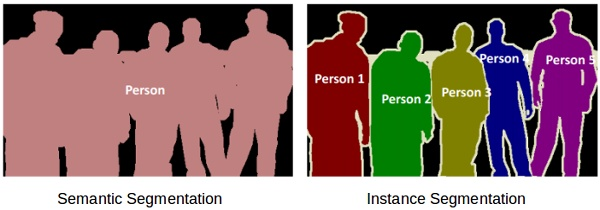
\includegraphics[width=0.7\linewidth]{figures/semanticVSinstance.jpg} 
  \caption{Semantic and Instance Segmentation. \cite{Varatharasan}}
  \label{fig:semanticVSinstance}
\end{figure}


Segmentation involves dividing an image into meaningful segments or regions. More precisely, segmentation can be divided into two types: semantic segmentation and instance segmentation. Semantic segmentation treats multiple objects within a single category as one entity. Instance segmentation, on the other hand, identifies individual objects within these categories \cite{ruiz2020semantic}. Within the realm of image forgery detection, semantic segmentation dominates the field as the segmentation task requires no further instance evaluation, in the sense that we only care about the tampered category and less about classifying the contents within it. The difference between the two is highlighted in Figure \ref{fig:semanticVSinstance} Traditional semantic segmentation techniques included thresholding, edge-based methods, and region-growing algorithms \cite{zhai2023background}. Thresholding assigns pixel values based on predefined intensity thresholds, while edge-based methods identify boundaries through gradient analysis \cite{huang2018weakly}. Region-growing algorithms group adjacent pixels with similar characteristics. Deep learning brought about a transformative shift in segmentation with Fully Convolutional Networks (FCNs) leading the way. FCNs utilize convolutional layers to capture spatial information and upsampling layers to generate dense pixel-wise predictions \cite{long2015fully}. U-Net, a popular architecture, combines a contracting path for context extraction and an expansive path for precise localization \cite{ronneberger2015unet}.

Recent state-of-the-art segmentation models often leverage the power of attention mechanisms. ViTs have been adapted for computer vision tasks, proving particularly effective for segmentation as they process images in the form of patch sequences, capturing global contextual information and enhancing segmentation accuracy \cite{strudel2021segmenter} \cite{thisanke2023semantic}.

In essence, while object localization initially addressed the question of `where' in computer vision, segmentation has expanded this understanding to the level of `what' and `how much' by delineating object boundaries at a finer granularity. The progression from bounding boxes to pixel-wise predictions showcases the iterative development of localization techniques that have influenced and contributed to the evolution of segmentation methods. In image forgery detection, these tasks become pivotal for unveiling the authenticity of images. Localization helps identify tampered regions within an image, while segmentation aids in precisely delineating the forged portions. By combining both techniques, one can achieve a comprehensive understanding of the manipulated areas, contributing to the development of robust forgery detection algorithms.

In the existing literature, there is an almost unanimous tendency to employ the term `localization' rather than `segmentation' when describing the methods applied in image forensics \cite{guo2023hierarchical} \cite{lai2023detect} \cite{Sharma2019} \cite{bunk2017detection} \cite{wang2019detection} \cite{Cozzolino2016} \cite{bianchi2011improved}. This linguistic choice often arises from a desire to convey a sense of pinpointing specific regions of interest within an image, while also encompassing the broader objective of identifying manipulated areas. While the true technical process involves segmentation, where regions are precisely delineated and differentiated, the term `localization' is employed to emphasize the goal of isolating and detecting forged regions without necessarily implying a detailed pixel-wise separation. This semantic shift in language reflects a pragmatic approach, simplifying the terminology for a wider audience and facilitating a more intuitive understanding of the primary objective - detecting and localizing image forgeries \cite{coulson2001semantic}. Following this approach, for alignment with the consensus, the term `localization' is used in this thesis in the same manner. 